\section{Design}
	\subsection{System Architecture Overview}
		The system will comprise of three main components:
		\begin{itemize}
			\item Management Server
			\item User Interface
			\item Disposable instances/containers
		\end{itemize}
		The system will also use existing infrastructure. This is where the backups are stored. Depending on the user of the system there may be multiple backup server in different location (such as AWS regions) or for different data types (relational and non-relational databases). Backup data may be stored in a variety of ways such as on EC2 instance or S3 buckets.
		
		\begin{figure}[H]
			\setlength{\belowcaptionskip}{15pt plus 3pt minus 2pt}
			\caption{Diagram of System Architecture}
			\centering
			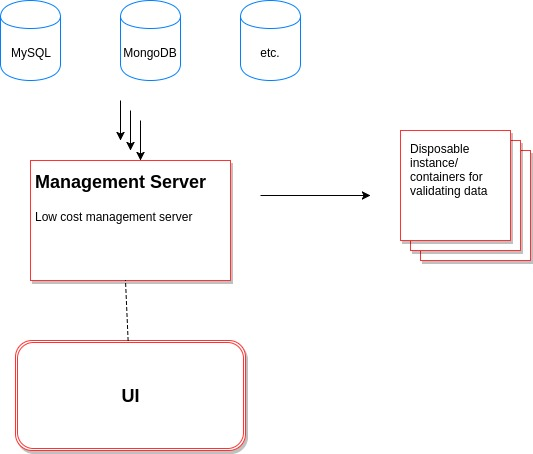
\includegraphics[scale=0.5,keepaspectratio]{diagram}
			\label{fig:diagram}
		\end{figure}
		
		\noindent \textbf{Management Server:} This will be a small low cost AWS instance on which the Jenkins automation server will be installed. The majority of the systems functionality will be carried out and/or orchestrated by this server. Jenkins jobs will copy the backups from their location to a disposable instance and implement the necessary steps to validate them such as importing and and reading.
		
		\noindent \textbf{User Interface:} This will provide a simple user interface (UI) for the system, implemented as a simple web app, hosted on AWS.It will allow users with little knowledge of Jenkins and AWS to perform backup restoration checks by adding a layer of abstraction. Users will be able to run restorations by providing the parameters such as the backup file and it's location. The UI will utilise the Jenkins API to run execute the restoration with the parameters provided.
		
		\noindent\textbf{Disposable Instances or Containers:} Disposable infrastructure will be used to perform the restoration. EC2 instances or containers can be used to quickly and easily deploy the necessary software to perform the restoration (i.e. the correct DB management system). They can also be destroyed afterwards, destroying the data and therefore maintaining confidentiality.

	\subsection{Formal Modelling}
	\subsubsection{Sequence Diagrams}
	
		The main function of the systems have been demonstrated below in sequence diagrams. \autoref{fig:seq-run-restore} shows the process of running a single backup restore. This involves a user manually triggering a restoration using the web interface. The trigger a Jenkins job automates the remaining steps. The backup is copied from the backup server to the test restoration server where it is imported to a Database Management System such as MongoDB. A read of the data is then performed to verify that the data is uncorrupted and readable. Finally it is destroyed from the restoration server.
		\begin{figure}[H]
			\setlength{\belowcaptionskip}{15pt plus 3pt minus 2pt}
			\caption{Run Restore}
			\centering
			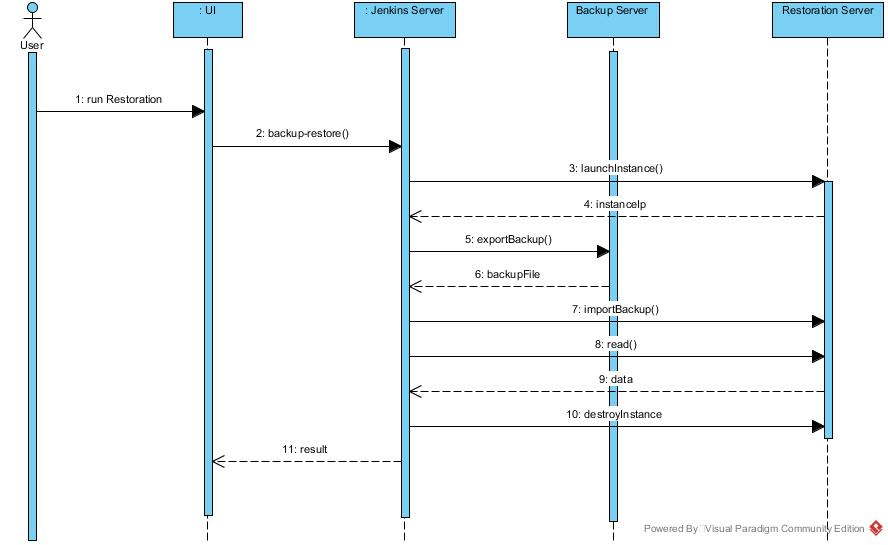
\includegraphics[width=\textwidth,keepaspectratio]{sequence-diagram-run-restore}
			\label{fig:seq-run-restore}
		\end{figure}

		\noindent \autoref{fig:seq-schedule-restore} shows the process of a scheduling regular backup restoration tests. Again, this is triggered by a user from the web interface. The web interface will pass the JSON or XML configuration for a job to the Jenkins server. The server will then create and save the job. A status indicating whether the job was created successfully is returned to the user. \note[id=RB]{Figure 3 is good too. Maybe here somewhere you could talk about what happens when the scheduled job runs - how does the user get notified about success/failure when they're not currently using the web app?}
		\begin{figure}[H]
			\setlength{\belowcaptionskip}{15pt plus 3pt minus 2pt}
			\caption{Schedule Regular Restore}
			\centering
			%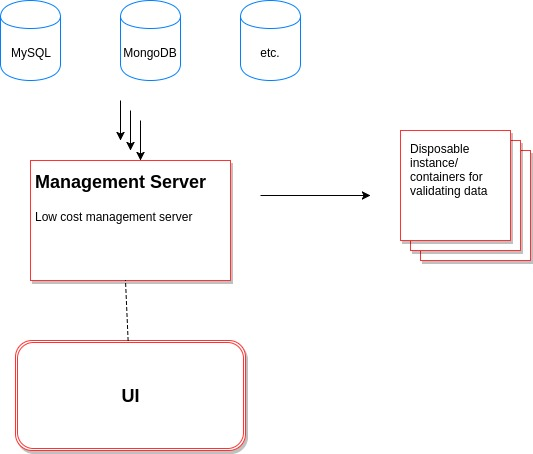
\includegraphics[width=\textwidth,height=\textheight,keepaspectratio]{diagram}
			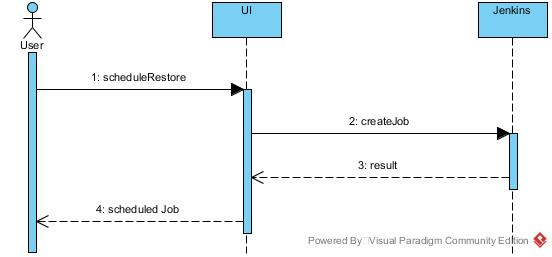
\includegraphics[width=\textwidth,keepaspectratio]{sequence-diagram-schedule-restore}
			\label{fig:seq-schedule-restore}
		\end{figure}
		
		\noindent \autoref{fig:seq-delete-restore} Show the process of deleting an existing scheduled job. This is required if a user not longer want to run scheduled restoration of a particular backup (for example if that backup is non longer needed and deleted). The user must delete the job on the Jenkins server in order to prevent further attempted restorations running. The user triggers this process from the web interface. This sends a delete commands to the Jenkins server via the API to remove the schedule job. The status of the command, indicating a successful or failed restore, is returned to the user. 
		\begin{figure}[H]
			\setlength{\belowcaptionskip}{15pt plus 3pt minus 2pt}
			\caption{Delete Scheduled Restore}
			\centering
			%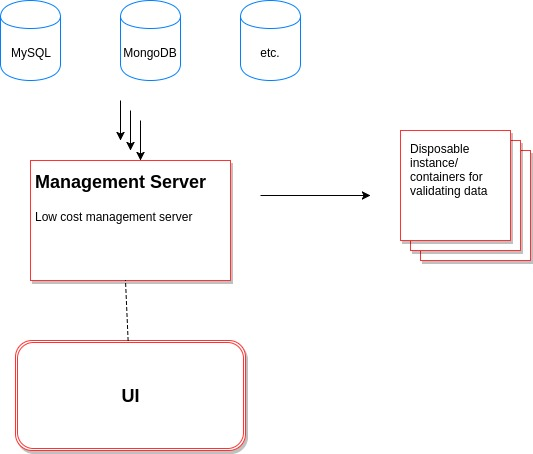
\includegraphics[width=\textwidth,height=\textheight,keepaspectratio]{diagram}
			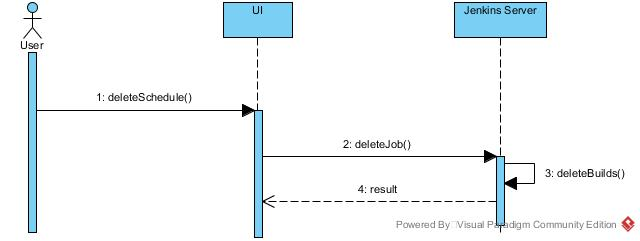
\includegraphics[width=\textwidth,keepaspectratio]{sequence-diagram-delete-schedule}
			\label{fig:seq-delete-restore}
		\end{figure}
	
	\subsubsection{User Stories}
		User stories are provided in \autoref{table:user-stories}. There are two users of the system; managers and users.
		
		Managers will have the ability to configure security aspects of the systems. This includes not only granting users access to the system but also adding credentials such as SSH keys and decryption keys. They will also be able to perform all the tasks that a regular user can perform without needing a set of regular user credentials.
		
		Regular users of the systems will be able to perform backup restoration after logging in. The will have the ability to run a restore at will and view the results. However, they will also be able to schedule the regular restoration of a backup and view the results of each restore that has occured.
		
		These the stories for general user such as running and scheduling restores. Also included are administration user stories. As system is create and destroys infrastructure on AWS, it would be necessary to limit access to the system.
		
		\begin{table}[H]
			\centering
			\setlength{\belowcaptionskip}{15pt plus 3pt minus 2pt}
			\caption{User Stories}
%			\begin{tabular}{|l|p{0.4\linewidth}|p{0.4\linewidth}|} \hline
			\begin{tabular}{|l|p{0.1\linewidth}|p{0.35\linewidth}|p{0.35\linewidth}|} \hline
				\textbf{\#} & \textbf{As a} & \textbf{I want to be able to} & \textbf{so that} \\ \hline
				US1 & manager & implement a user system & I control who can run backup restores \\ \hline
				US1.1 & manager & add my team members to the system & they can run backup restores \\ \hline
				US1.2 & manager & remove users from the system & former team members no longer have access \\ \hline
				US2 & manager & add and control sensitive information within the system & I can implement a security policy \\ \hline
				US2.2 & manager & securely store credentials within the system & they don't need to be entered every time a restore is executed \\ \hline
				US2.3 & manager & add SSH keys for backup server & the system has secure access backup server \\ \hline
				US2.4 & manager & add decryption keys for backups & encrypted backups can be decrypted for testing \\ \hline
				US2.5 & manager & delete SSH keys & expired/outdated credentials are no longer stored \\ \hline
				US2.6 & manager & delete decryption keys & expired/outdated credentials are no longer stored \\ \hline
				US3 & manager & execute all same tasks as a regular user & I don't need a second set of credentials to run restores myself \\ \hline
				US4 & user & login & I can run restores \\ \hline
				US5 & user & logout & I avoid potential unauthorised access \\ \hline
				US6 & user & run a test restoration of a backup & I can verify that the backup exists, is a valid file, and is readable \\ \hline
				US6.1 & user & run a test by filling out a simple form with basic parameters (location, filename) of the backup to test & I can easily run a restore of a specific backup without needing to worry about the implementation \\ \hline
				US6.2 & user & view the current status a running restoration & I can review the progress of long running restores \\ \hline
				US6.3 & user & check if a backup failed or succeeded & I can immediately investigate any failed backups \\ \hline
				US7 & user & create a schedule of automated restores for a given backup & I don't have to manually execute them myself on a regular basis \\ \hline
				US7.1 & user & choose the frequency of automated restores within a schedule, from daily through weekly to monthly & I control how often different backups are tested \\ \hline
				US7.2 & user & check if an automated restoration has started & I can verify my schedule is working correctly \\ \hline
				US7.3 & user & check the results of an automated restore & I can immediately investigate any failed backups \\ \hline
				US7.4 & user & view the all past results of an automated restore schedule & view the consistency of my backups success \\ \hline
				US7.5 & user & modify a scheduled restore & I can change the frequency of a scheduled restore \\ \hline
				US7.6 & user & the parameters of a schedule & any changes to the backups, such as location, will be reflect in the restoration schedule \\ \hline
				US7.7 & user & delete regularly scheduled restores & old backups/deleted backups are no longer tested \\ \hline
				US8 & user & view feedback of a failed restore & I might gain an insight into the fault in the backup \\ \hline
				US9 & user & notified when a restoration fails & silent, unnoticed fails are avoided \\ \hline
			\end{tabular}
			\label{table:user-stories}
		\end{table}
		
	\subsection{Front End Design}
	\subsubsection{Wireframes}
		\begin{figure}[H]
			\setlength{\belowcaptionskip}{15pt plus 3pt minus 2pt}
			\caption{Homepage}
			\centering
			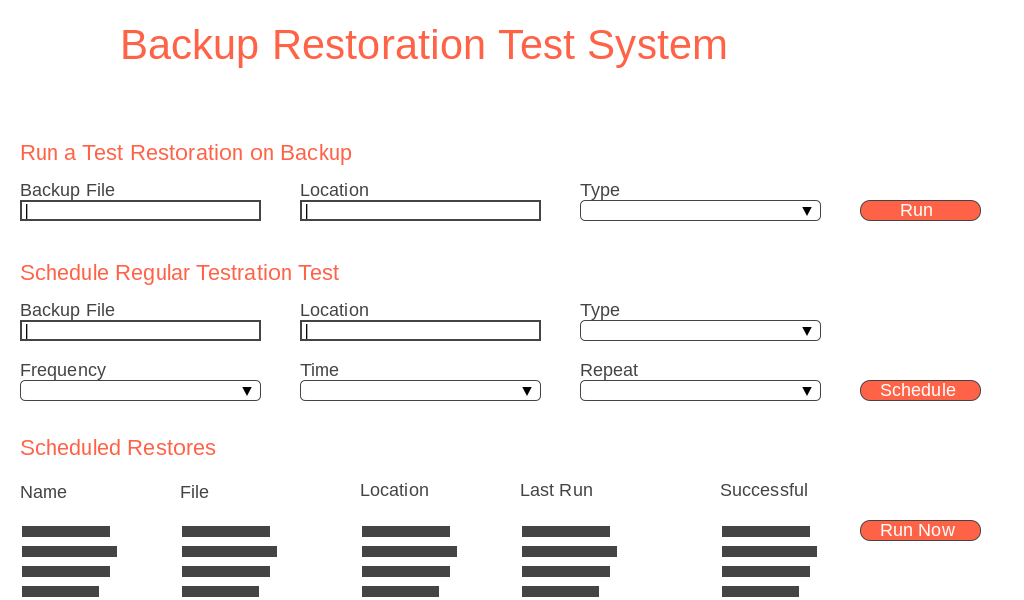
\includegraphics[width=\textwidth,keepaspectratio]{wireframe-homepage}
			\label{fig:homepage}
		\end{figure}
		
		\begin{figure}[H]
			\setlength{\belowcaptionskip}{15pt plus 3pt minus 2pt}
			\caption{Scheduled Restore}
			\centering
			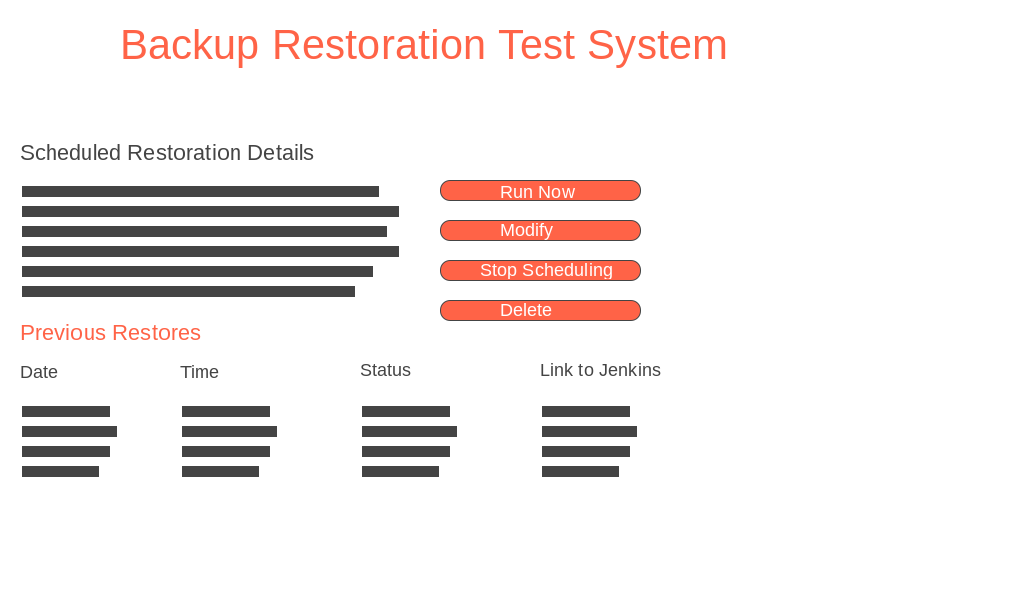
\includegraphics[width=\textwidth,keepaspectratio]{wireframe-scheduled-restore}
			\label{fig:scheduled}
		\end{figure}
	